 
\section{ECAL Data Format}\label{sec:ECAL}

The ECAL data are composed by 54 event fragments processed in the Data
Concentrator Card (DCC) boards~\cite{LECC03,CALOR04} (36 for the ECAL Barrel (EB) and 18 for
the ECAL End-Cap (EE)). 
The ECAL raw data format is shown in Table~\ref{tab:ECAL}. 
Each Event is composed of five block types:
\begin{itemize}
\item   DCC Header Block
\item   TCC Block
\item   SR Block
\item   Tower Block
\item   Crystal Block
\end{itemize}
These blocks are organized in 64 bit words and are enclosed by the standard CMS DAQ header and trailer. Each block is characterized by a unique bit field identifier, which helps to track possible data formatting errors.

\begin{table}[htp]
\caption{The ECAL data format.}
\label{tab:ECAL}
  \hspace{-0.11\linewidth}
  \begin{minipage}{1.22\linewidth}
  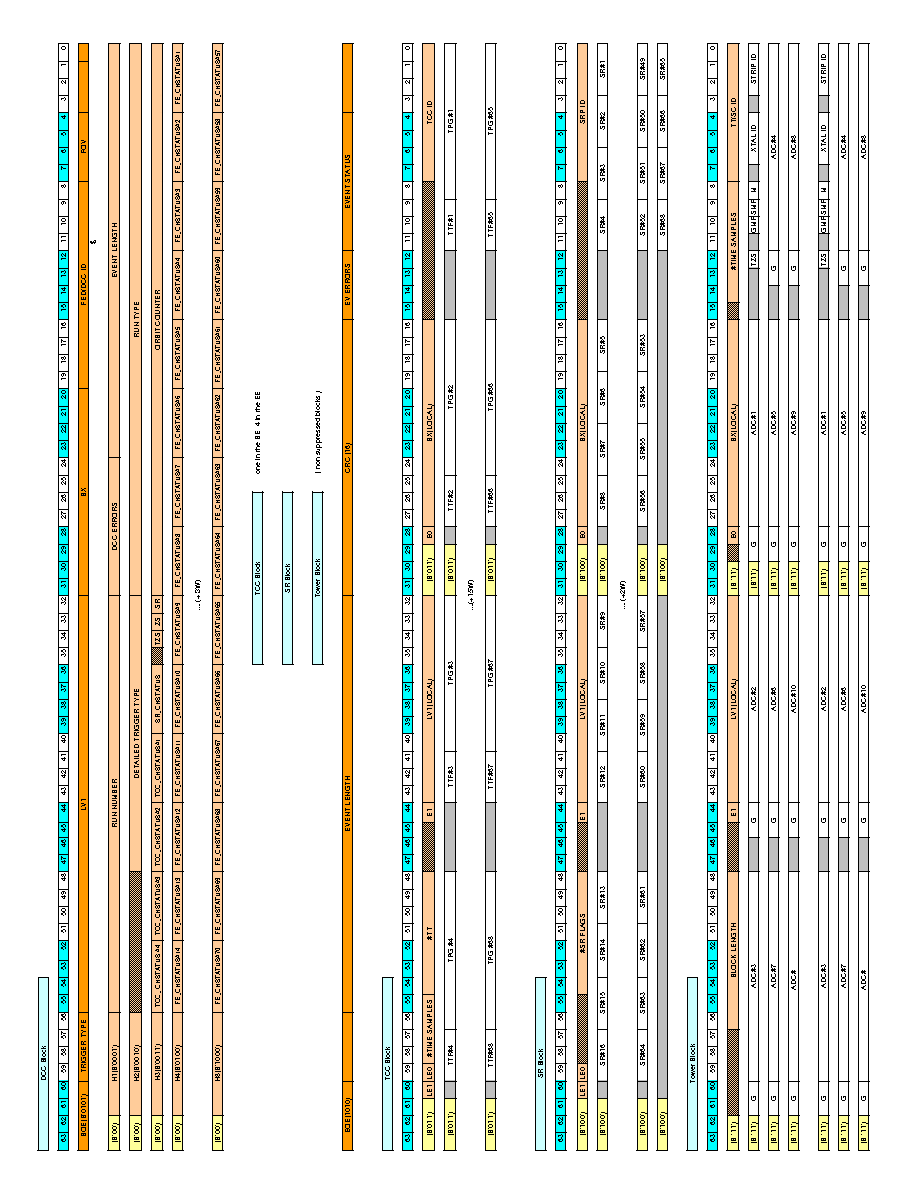
\epsfig{file=ECAL,width=\linewidth}
  \end{minipage}
\end{table}

The data structure starts with the standard CMS DAQ header followed by the specific ECAL DCC Header Block. Trigger data received from the Trigger Concentrator Card (TCC)~\cite{CALOR04} are grouped in the TCC Blocks. The number of TCC Blocks depends on the detector geometry, being one in the EB and four in the EE. 
Front-End (FE) data must be reduced by a factor of near 20. ECAL data filtering is based on a Selective Readout algorithm finding ECAL areas of interest, which should be readout with low zero suppression or without zero suppression at all. The other areas can be suppressed or readout with a higher zero suppression level. For each readout unit, comprising a Trigger Tower in the EB geometry or a Super Crystal in the EE geometry, there is a flag identifying the level of data suppression that must be applied to the input data. These flags are processed in the Selective Readout Processor (SRP)~\cite{CALOR04,IEEE04} and grouped in the SR Block.
The number of Tower (or Super Crystal) Blocks in each event depends on the enabled FE channels and on the SR flags, which can suppress the entire FE channel data. The number of Crystal Blocks belonging to a given Tower Block (or Super Crystal) is dynamic and depends on the deposited energy and on the associated SR flag.

\subsection{DCC Header Block}

The DCC Header Block is composed by eight words characterized by a block identifier (B'00') and a header word number (from 1 to 8). The block carries the following fields:
\begin{description}
\item {\bf EVENT LENGTH}: Number of 64 bit words in the event, also present
  in the CMS DAQ trailer. This number includes the CMS DAQ header and trailer
  words. The fact that the event length is placed at the beginning of the event makes it more suitable for a fast decoding and event characterization.
\item {\bf DCC ERRORS}: The DCC event error field described in 
Table~\ref{tab:DCCerror}.
\item {\bf RUN NUMBER}: Sequential run number or encoded run conditions as written in the DCC Run ID register.
\item {\bf Hi}: Header word count identifier.
\item {\bf RUN TYPE}: Field (Table~\ref{tab:ECAL_RunType}) encoded by the DCC supervisor software in local data taking mode and written into the DCC Run Type register.
\begin{description}
\item[-] {\bf RT\_DCCID}:  The DCC ID;
\item[-] {\bf RT\_HALF}: Part of the Super module to be readout (Table~\ref{tab:RT_HALF}).
\item[-] {\bf RT\_TYPE}: The run type (Table~\ref{tab:RT_TYPE}).
\item[-] {\bf SEQUENCE}: The operation sequence during a local run. The SEQUENCE encoding depends on the RT\_TYPE and its description is shown in Table~\ref{tab:SEQUENCE}.
\item[-] {\bf MGPA GAIN}: The MPGA operation gain mode during the local run (Table~\ref{tab:MGPAG}).
\item[-] {\bf MEM GAIN}: The MEM channels operation gain mode during the local run (Table~\ref{tab:MGPAM}).
\item[-] {\bf CYCLE SETTINGS}: The cycle operation settings applied during the local run. The CYCLE SETTINGS encoding depends on the SEQUENCE and is shown in Table~\ref{tab:ECAL_RunType}. The POWER, FILTER, DELAY, VINJ, MGPA CONTENT and OFFSET fields are binary representations of configuration parameters for each SEQUENCE type. The RT\_WL field encodes the Laser/LED wavelength according to Table~\ref{tab:RT_WL}.
\end{description}
\item {\bf DETAILED TRIGGER TYPE}: A Timing and Trigger Control (TTC)~\cite{ELHC00}
  long command that is written in the DCC header during calibration triggers
  in the orbit gaps. The content of this word is the following:
\begin{description}
\item[-] {\bf DTT\_DCCID}: The DCC ID
\item[-] {\bf DTT\_HALF}:  The same as RT\_HALF (Table~\ref{tab:RT_HALF}).
\item[-] {\bf DTT\_TYPE}: The same as RT\_TYPE (Table~\ref{tab:RT_TYPE}).
\item[-] {\bf DTT\_WL}: The same as RT\_WL (Table~\ref{tab:RT_WL}).
\end{description}
\item {\bf ORBIT COUNTER}: The orbit number in the run.
\item {\bf SR and ZS}: These bit fields characterize the DCC readout conditions. The SR bit specifies if selective readout is enabled and in the case of being disabled the ZS field specifies if crystal data must be zero suppressed or fully readout.
\item {\bf TZS}: Test Zero Suppression mode. In this operation mode (TZS=1) the zero suppression (if requested in the DCC configuration or by a SR flag) is applied to the crystal data without data removal. The result of the filter is set in the TZS field of the Crystal Block allowing testing off-line the ZS algorithm.
\item {\bf SR\_CHSTATUS}: SRP input channel status (Table~\ref{tab:CHSTATUS}).
\item {\bf TCC\_CHSTATUS\#i}: TCC input channel \#i status (Table~\ref{tab:CHSTATUS}).
\item {\bf FE\_CHSTATUS\#i}:  FE input channel \#i status (Table~\ref{tab:CHSTATUS}).
\end{description}

\begin{table}[htp]
\begin{center}
\caption{DCC error description.}
\label{tab:DCCerror}
\begin{tabular}{|c|l|} \hline
{\bf DCC Error} (binary) &      {\bf Description} \\ \hline
00000000 &      No Errors \\ \hline
00000001 &      Empty event produced : 
 DAQ header + the first two DCC header words + DAQ trailer \\ \hline
xxxxxx1x &      Data timeout : at least one channel has a data presence
timeout \\ \hline
0xxxx1xx &      Channel error: at least one channel on error \\ \hline
? &     To be defined \\ \hline
1xxxxxxx &      No error  check performed \\ \hline
\end{tabular}
\end{center}
\end{table}
 
\begin{table}[htp]
\begin{center}
  \caption{The Run Type word format. The CYCLE SETTINGS encoding depends on the selected SEQUENCE.}
  \label{tab:ECAL_RunType}
  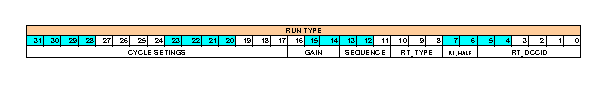
\epsfig{file=ECAL_RunType,width=\linewidth}
 \end{center}
\end{table}

\begin{table}[htp]
\begin{center}
\caption{RT\_HALF description.}
\label{tab:RT_HALF}
\begin{tabular}{|c|l|} \hline 
{\bf RT\_HALF}  (binary)        & {\bf Description} \\ \hline
01 &    First super module half  \\ \hline
10 &    Second super module half \\ \hline
11 &    Full super module \\ \hline
\end{tabular}
\end{center}
\end{table}

\begin{table}[htp]
\begin{center}
\caption{RT\_TYPE description.}
\label{tab:RT_TYPE}
\begin{tabular}{|c|l|}  \hline
{\bf RT\_TYPE}  (binary)        & Description \\ \hline
001 &   Laser \\ \hline
010 &   Test Pulse \\ \hline
011 &   Pedestal \\ \hline
100 &   LED \\ \hline
\end{tabular}
\end{center}
\end{table}

\begin{table}[htp]
\begin{center}
\caption{SEQUENCE description.}
\label{tab:SEQUENCE}
\begin{tabular}{|c|l|}  \hline 
{\bf SEQUENCE} (binary) & Description  \\ \hline
\multicolumn{2}{l}{If  RT\_TYPE is Laser Trigger} \\ \hline
000 &   Standard Laser  \\ \hline
001 &   Laser Power Scan  \\ \hline
010 &   Delay Scan  \\ \hline
\multicolumn{2}{l}{If RT\_TYPE is Test Pulse Trigger} \\ \hline
000 &   Scan MEM \\ \hline
001 &   MGPA \\ \hline
\multicolumn{2}{l}{If RT\_TYPE is Pedestal} \\ \hline
000 &   Standard Pedestal \\ \hline
001 &   Pedestal Offset Scan \\ \hline
\multicolumn{2}{l}{If RT\_TYPE is LED} \\ \hline
000 &   Standard LED \\ \hline
\end{tabular}
\end{center}
\end{table}

\begin{table}[htp]
\begin{center}
\caption{MGPA gain description.}
\label{tab:MGPAG}
\begin{tabular}{|c|l|}   \hline  
{\bf MGPA} (binary) &   Description \\ \hline
00 &    Free gain (default) \\ \hline
01 &    Forced gain 12 \\ \hline
10 &    Forced gain 6 \\ \hline
11 &    Forced gain 1 \\ \hline
\end{tabular}
\end{center}
\end{table}

\begin{table}[htp]
\begin{center}
\caption{MEM gain description.}
\label{tab:MGPAM}
\begin{tabular}{|c|l|}   \hline 
{\bf MEM} (binary) &    Description \\ \hline
0 &     MEM forced gain 1 \\ \hline
1 &     MEM forced gain 16 (default) \\ \hline
\end{tabular}
\end{center}
\end{table}

\begin{table}[htp]
\begin{center}
\caption{ The RT\_WL description.}
\label{tab:RT_WL}
\begin{tabular}{|c|l|}   \hline 
{\bf RT\_WL} (binary) & Description \\ \hline
001 &   Red (Laser) \\ \hline
010 &   Blue (Laser) \\ \hline
011 &   Infra-Red (Laser) \\ \hline
100 &   Green (Laser) \\ \hline
101 &   $\lambda$1 (LED) \\ \hline
110 &   $\lambda$2 (LED) \\ \hline
\end{tabular}
\end{center}
\end{table}

\begin{table}[htp]
\begin{center}
  \caption{Detailed trigger type word format.}
  \label{tab:ECAL_detailedTriggerType}
  
\epsfig{file=ECAL_detailedTriggerType,width=0.75\linewidth}
\end{center}
\end{table}

\begin{table}[htp]
\begin{center}
\caption{DCC Channel status description. If multiple errors are
  identified the channel status is set according to its priority 
(a lower channel status value implies a higher priority).}
\label{tab:CHSTATUS}
\begin{tabular}{|c|l|}   \hline  
{\bf CHSTATUS } &       Description \\ \hline
0000 &  Channel enabled and no errors identified   \\ \hline
0001 &  Channel disabled by configuration \\ \hline
0010 &  Channel data ignored in response to a data presence timeout \\ \hline
0011 &  Header identifier mismatch \\ \hline
0100 &  Block word count mismatch \\ \hline
10xx &  Sync error (bit 0: LV1 , bit 1: BX) \\ \hline
11xx &  Parity error  (bit 0: horizontal parity , bit 1 : vertical parity) \\ \hline
\end{tabular}
\end{center}
\end{table}

\subsection{TCC Block}
 
The TCC Blocks, added after the DCC Block Header, include the trigger data received from the TCC links. The bock is identified by the B('011') field at the beginning of each 32 bit word and is composed by the following fields: 
\begin{description}
\item {\bf TCC ID}: The trigger data source board id (from 1 to 108).
\item {\bf BX}: TCC local bunch crossing (BX) counter.
\item {\bf E0}: DCC BX error bit (active if there is a mismatch between the TCC BX counter and the DCC BX counter).  
\item {\bf LV1}: TCC local level one accept (LV1) counter.
\item {\bf E1}: DCC LV1 error bit (active if there is a mismatch between the TCC LV1 counter and the DCC LV1 counter).
\item {\bf \#TT}: Number of Trigger Towers (TTs) associated to this TCC. In the EB each TCC is associated to 68 TTs. In the inner EE each TCC Block includes a maximum of 32 TTs words while in the outer EE this number is decreased to 16. An EE DCC serves two 20 degrees sectors with two inner and two outer EE sections. 
\item {\bf \#TIME SAMPLES}: Number of time samples for the Trigger Primitives Generator (TPG) data words. In normal data acquisition mode there is only one time sample. For debugging operation mode, 4 or 8 time samples are foreseen. For multiple time samples, TT flags and TPG data are ordered consecutively per set of samples in each TT.
\item {\bf LE0}: Local BX error bit. This bit is received from the TCC data and identifies if there is a mismatch (LE0=1) between the TCC local BX counter and the info received from the TTC system.
\item {\bf LE1}: Local LV1 error bit. This bit is received from the TCC data and identifies if there is a mismatch (LE1=1) between the TCC local LV1 counter and the info received from the TTC system.
\item {\bf TPG\#i}: 9 bits coding the trigger primitive of TT i.
\item {\bf TTF\#i}: TT flag (Table~\ref{tab:TTFlag}) sent from the TCC to the SRP and included in the DCC for debugging proposes. The first two bit flags characterize the TT energetic state, while the third bit is enabled if the TT flag was produced with erroneous conditions. 
\end{description}

\begin{table}[htp]
\begin{center}
\caption{Trigger tower flags description.}
\label{tab:TTFlag}
\begin{tabular}{|c|l|} \hline
{\bf TT Flag} & Description \\ \hline
000 &   Low interest TT (Tower Et is bellow low threshold) \\ \hline
001 &   Mid-interest TT (Tower Et is between low and high thresholds) \\ \hline
010 &   Not used \\ \hline
011 &   High-interest TT (Tower Et is above high threshold) \\ \hline
100 &   Force TT readout (Agilent sync link error ) \\ \hline
101 &   Force TT readout (Hamming code error ) \\ \hline
11x &   Force TT readout (Other error conditions )  \\ \hline
\end{tabular}
\end{center}
\end{table}

\subsection{SRP Block}
 
The SRP Block, added after the TCC Blocks, includes the selective readout flags received from the SRP link. The block is identified by the B(�100�) field at the beginning of each 32 bit word and is composed by the following fields:
\begin{description}
\item {\bf SRP ID}: The SRP identification.
\item {\bf BX}: SRP local BX counter.
\item {\bf E0}: DCC BX error bit (active if there is a mismatch between the SRP BX counter and the DCC BX counter).  
\item {\bf LV1}: SRP local LV1 counter.
\item {\bf E1}: DCC LV1 error bit (active if there is a mismatch between the SRP LV1 counter and the DCC LV1 counter).
\item {\bf \#SRFLAGS}: Number of SR flags associated to this link. In the EB the DCC receives a total of 68 SR flags, while in the EE the DCC receives 34, 35 or 36 flags.  
\item {\bf LE0}: Local BX error bit. This bit is received from the SRP data and identifies if there is a mismatch (LE0=1) between the SRP local BX counter and the info received from the TTC System.
\item {\bf LE1}: Local LV1 error bit. This bit is received from the SRP data and identifies if there is a mismatch (LE1=0) between the SRP local LV1 counter and the info received from the TTC System.
\item {\bf SR\#i}: 3 bits coding the SR flags for each FE channel (Table~\ref{tab:SRPFlag}). The first two bit flags characterize the SRP algorithm flag, while the third bit is used to indicate if the flag was produced in erroneous conditions.
\end{description}

\begin{table}[htbp]
\begin{center}
\caption{Selective Readout flags description.}
\label{tab:SRPFlag}
\begin{tabular}{|c|l|}   \hline 
{\bf SR Flag} & Description  \\ \hline
000 &   Suppress FE channel  \\ \hline
001 &   Read FE channel with lv1 zero suppression   \\ \hline
010 &   Read FE channel with lv2 zero suppression  \\ \hline
011 &   Read FE channel without zero suppression  \\ \hline
1xx &   xx action has been forced by an erroneous condition or by configuration:  \\ 
    & - TT flagged in forced readout mode (from TCC)  \\
    & - Data transmission errors (TCC and Algorithm Board(AB) link errors)  \\ \hline
\end{tabular}
\end{center}
\end{table}

\subsection{Tower Header and Crystal Blocks}

The Tower Block collects filtered FE data received from the FE boards, and is organized in Crystal Blocks. The Tower (or Super Crystal in the EE) Block contains a maximum of 25 crystals, corresponding to a fully readout tower (or super crystal). The Tower Blocks and the Crystal Blocks are identified by the B(�11�) field at the beginning of each 32 bit word and are composed by the following fields:
\begin{description}
\item {\bf Tower Header Block}:
\begin{description}
\item {\bf TT/SC ID}: The FE readout board id (from 1 to 68).
\item {\bf \#TIME SAMPLES}: Number of time samples for the ADC crystal data (default is 10). The number of samples accepted by the DCC is given by:  2 +4n (where n goes from 0 to 15).
\item {\bf BX}: FE local BX counter.
\item {\bf E0}: DCC BX error bit (active if there is a mismatch between the FE BX counter and the DCC BX counter).  
\item {\bf LV1}: FE local LV1 counter.
\item {\bf E1}: DCC LV1 error bit (active if there is a mismatch between the FE LV1 counter and the DCC LV1 counter).
\item {\bf BLOCK LENGTH}: A block word counter, in 64 bit words, tacking into account the Tower Header Block and the Crystal Block words.
\end{description}
\item {\bf Crystal Block}:
\begin{description}
\item {\bf STRIP ID}: The crystal strip identification (from one to five).
\item {\bf CRYSTAL ID}: The crystal identification inside the strip (from one to five).
\item {\bf M}: Monitoring bit, enabled for monitoring triggers.
\item {\bf GMF and SMF}: bit fields received from the FE strip header (see Annex A.1), the GM flag and the SM flag qualify respectively a Global or a Strip level crystal time sample misalignment.
\item {\bf TZS}: When the DCC is configured to operate in the test zero suppression mode, the TZS bit will be enabled whenever the crystal data frame is flagged to be suppressed.
\item {\bf ADC\#i}: 12 bits representing the crystal time sample i. 
\item {\bf G}:  MGPA gain (B'00': not used, B'01': gain 12, B'10': gain 6, B'11': gain 1). 
\end{description}
\end{description}

The crystal numbering in the DCC raw data format follows the FE numbering scheme. The FE identifies each crystal by the strip to which it belongs to (from one to five) and the crystal number inside the strip (from one to five). To get the absolute crystal number inside the TT or inside the Super Module, a lookup table should be applied. The lookup table should take into account the particular arrangement of VFE cards inside the FE card, and the particular arrangement of FE cards inside the Super Module. 


%%% NA:  The content of this section is already present in Section 2.
%\subsection{CMS DAQ Header and Trailer}

%The CMS DAQ Header and trailer~\cite{TRIDAS} are respectively the first and last word of the ECAL event represented in Table~\ref{tab:ECAL}.

%The DAQ Header includes the fields:
%\begin{description}     
%\item {\bf \$}: Bit used by the S-Link 64 hardware.
%\item {\bf H}: Header bit. When set to '0', the current header word is the last one. When set to '1', other header word can follow (in the ECAL DCC, H is set to �1� ). 
%\item {\bf FOV}: Version identifier of the FED/DCC data format.
%\item {\bf FED/DCC ID}: The Front End Driver identification, corresponding to the DCC id (from 1 to 54).
%\item {\bf BX}:  Bunch crossing counter (from the TTC System).
%\item {\bf LV1}:  Level one accept counter (from the TTC System).
%\item {\bf TRIGGER TYPE}: Event Trigger Type, defined by the central DAQ and
%  shown in Table~\ref{tab:TRIGGER_TYPE}~\cite{NOTE_2002/033}. 
%\item {\bf BOE}: Begin of event bit field identifier with value B('0101').
%\end{description}

%\begin{table}[htp]
%\begin{center}
%\caption{The TRIGGER TYPE description.}
%\label{tab:TRIGGER_TYPE}
%\begin{tabular}{|c|l|}   \hline 
%{\bf TRIGGER TYPE} &    Description \\ \hline
%0001 &  Physics trigger \\ \hline
%0010 &  Calibration trigger \\ \hline
%0011 &  Test trigger \\ \hline
%0100 &  Technical trigger (external trigger) \\ \hline
%0101 &  Simulated events (reserved for DAQ usage) \\ \hline
%0110 &  Traced events (reserved for DAQ usage) \\ \hline
%1111 &  Error \\ \hline
%\end{tabular}
%\end{center}
%\end{table}

%The DAQ Trailer includes the fields:
%\begin{description}     
%\item {\bf \$}: Bit used by the S-Link 64 hardware.
%\item {\bf T}: Trailer bit. When set to '0', the current trailer word is the last one. When set to �1�, other trailler words can fallow, (in the ECAL DCC, T is set to 0 ).
%\item {\bf TTS}: Current Trigger Throttling System bits. 
%\item {\bf EVENT STATUS}: Event fragment status (defined by the central DAQ).
%\item {\bf CRC}: Cyclic Redundancy Code of the event fragment including header and trailer.
%\item {\bf EVENT LENGTH}: The same meaning has the Event Length in the DCC Header Block.
%\item {\bf EOV}: End of event bit field identifier with value B('1010')
%\end{description}

\subsection{Erroneous input data and implications on ECAL Raw data}

The identification of erroneous input data fragments has implications on the
way the event is built. The actions taken from the DCC in
presence of erroneous input data are described in this section. 
\begin{description}
\item {\bf Synchronization error with erroneous BX or LV1 from an input channel}:
\begin{description}
\item[-] Global action: The channel data are included in the assembled event and the associated channel status field set with the sync error flag.
\item[-] Error identified in the SRP Block: No filtering is applied to crystal data.
\item[-] Error identified in the FE Block: No filtering is applied to crystal data from this particular channel.
\end{description}
\item {\bf Data timeouts, wrong header identifiers or block word counts}:
\begin{description}
\item[-] These are considered severe errors. Data from the faulty channel are ignored and the channel status is flagged with the identified error condition. 
\end{description}
\item {\bf Misaligned FE Data (GMF or SMF bits)}:
\begin{description}
\item[-] The crystal data with misaligned time samples are not zero suppressed.
\end{description}
\end{description}
The DCC is also able to operate with no error check (DCCERR set to
'1xxxxxxxx').

\subsection{Raw Data Parsing and Monitoring}

Detector raw data need to be decoded and the data quality monitored. In the Off-line system data will serve physics analysis, while in the On-line system local data taking is used mainly to monitor the detector performance.
A software package was developed with the intent to allow on-line and off-line applications to access all defined raw data bit fields in an object oriented way. In addition, the package verifies the event data structure identifying possible errors. The class diagram for this package, developed in C++, is represented in Figure 4.

Figure 4. The data parser class diagram.

Raw data blocks are characterized by a set of bit fields. Each bit field is defined through a word position inside the block, a bit position inside the word and a defined bit size. The DCCDataField class is a representation of a raw data bit field. These data structures are built and stored in the DCCDataMapper containers. The DCCDataBlockPrototype class encapsulates the knowledge on how to decode a raw data buffer based on the defined bit fields. When parsing the input data buffers the decoded bit fields are stored in a map container, which can be accessed by the applications using the parser. During the parsing process the DCC data blocks classes perform a set of checks on the decoded data. These checks are described in Table~\ref{tab:error_check}.
The information about the blocks that need to be created is stored in the data itself. The DCCEventBlock decodes the DCC header bit fields identifying the enabled channels. In a first stage the blocks associated to the enabled TCC and SR channels are created. The DCCTowerBlock instantiation is based on the enabled FE channels and on the SR flags that indicate the rejected channels. The size of the DCCTowerBlock and the knowledge of the number of time samples per crystal allow the determination of the number of readout crystals in each tower or super crystal. For each crystal is instantiated a DCCXtalBlock object. The parsing ends up with the decoding of the DCC trailer. The software includes methods that allow the event raw data display in function of the defined bit fields.
The package describing the 2004 H4 Test Beam ECAL raw data is implemented and is included in ORCA\_8\_8\_0~\cite{ORCA} (Calorimetry/EcalBarrelTBDaqDigiFormat). The package is responsible by decoding the raw data and by generating the Calo Data Samples Frames.

\begin{table}[htbp]
\begin{center}
\caption{Error checks performed during parsing.}
\label{tab:error_check}
\begin{tabular}{|c|p{108mm}|}   \hline  
{\bf Data Block} &      Error check description \\ \hline
DCCEventBlock & Begin Of Event, header identifiers and block identifier \\ \hline
DCCTCCBlock &   Channel id, synchronization and block identifiers \\ \hline
DCCSRPBlock &   Channel id, synchronization and block identifiers \\ \hline
DCCTowerBlock & Channel id, synchronization, block identifiers and block size (based on the readout conditions and number of crystal samples) \\ \hline
DCCCrystalBlock & Crystal and strip ids and block identifiers \\ \hline
DCCTraillerBlock & End Of Event, event size and CRC \\ \hline
\end{tabular}
\end{center}
\end{table}




%%% Local Variables: 
%%% mode: latex
%%% TeX-master: "DataFormats"
%%% End: 
%{\textwidth}
